\documentclass[a4paper, 12pt, finnish]{article}
\usepackage{babel}
\usepackage[utf8]{inputenc}
\usepackage[T1]{fontenc}
\usepackage{graphicx}
\usepackage{caption}
\captionsetup{labelformat=empty}
\title{Keskustelufoorumin Dokumentaatio}
\author{Timo Mäki}
\date{\today}

\begin{document}
 \maketitle

Tämä on dokumentaatio tietokantasovelluksen harjoitustyön keskustelufoorumiin.

\newpage\null\thispagestyle{empty}\newpage
\tableofcontents
\newpage\null\thispagestyle{empty}\newpage
\section{Johdanto}

Aiheena on luoda keskustelufoorumi.
Foorumissa käyttäjät voivat kirjoittaa viestejä ja lukea muiden kirjoittamia viestejä.
Viestit liittyvät viestiketjuihin, joilla on otsikoita.
Käyttäjät voivat luoda viestiketjuja.
Viestejä voi etsiä viestin ajan, aiheen ja kirjoittajan perusteella.
Käyttäjillä on yksityiset tunnukset, joilla he voivat kirjautua sisään.
Tunnukset tarvitaan, jotta voi kirjoittaa viestejä foorumille.
Jokaisella käyttäjätunnuksella voi kirjoittaa viestejä.
Pääkäyttäjällä on oikeus viedä käyttäjän oikeus kirjoittaa viestejä, sekä muokkaa viestejä, että viestiketjuja sekä poistaa jälkimmäisiä.
\indent

Foorumin tarkoitus on edistää sosiaalista kanssakäyntiä ihmisten välillä, auttaa samanhenkisiä ihmisiä löytämään toisensa ja antaa ihmisten sekä anonyymisti että toisia kunnioittavasti esittää mielipiteitään internetin välityksellä.
\indent

Järjestelmän tavoitteet ovat mahdollistaa viestien kirjoitus ja luku, käyttäjätunnusten luonti, käyttöoikeusryhmien olemassaolo sekä mahdollistaa nopea viestin haku.
\indent

Järjestelmä pyörii tktl:n users palvelimella, apachea käyttäen.
Se vaatii PHP-tuen.
Käyttäjän selaimelta ei edellytetä tukea javascriptille, mutta HTML5 tuki edellytetään.
Järjestelmä edellyttää PostgreSQL tietokantaa.
On todennäköistä, että, rajapintoja hyödyntäen, tietokanta tulee olemaan jokseenkin helppo vaihtaa.

\newpage
\section{Yleiskuva järjestelmästä}
\subsection{Jokamies}
Jokamies on henkilö, joka ei ole välttämättä rekisteröitynyt tai kirjautunut sisään.
Jokainen foorumin käyttäjä on jokamies.

\begin{itemize}
\item
Voi lukea foorumille tehtyjä kirjoituksia.

\item
Voi hakea viestejä.

\item
Voi rekisteröityä.

\item
Voi kirjautua foorumiin.
\end{itemize}

\subsection{Rekisteröitynyt käyttäjä}
Rekisteröitynyt käyttäjä on henkilö, joka on rekisteröinyt tunnuksen foorumille.
Rekisteröitynyt käyttäjä on myös jokamies.

\begin{itemize}
\item
    Voi aloittaa uuden viestiketjun.
\item
    Voi vastata olemassa olevaan viestiketjuun.
\item
    Näkee kirjoitukset, joita henkilö ei ole vielä lukenut.
\item
    Voi muokkaa omia viestejään.
\end{itemize}

\subsection{Pääkäyttäjä}
Pääkäyttäjä on henkilö, joka vastaa foorumin ylläpidosta.
Tämä on erityisryhmä ja on oletusarvoisesti vain foorumin perustajalla. Pääkäyttäjällä on myös rekisteröityneen käyttäjän oikeudet.

\begin{itemize}
\item
Voi muokkaa viestiketjuja sekä kaikkia viestejä.
\item
Voi poistaa foorumille kirjoitetun viestiketjun.
\item
Voi laittaa eston käyttäjälle, jolloin tämä ei voi enää kirjoittaa uusia viestejä foorumille.
\item
Voi antaa pääkäyttäjän oikeudet muille rekisteröityneille käyttäjille.
\end{itemize}

\subsection{Viestikiellossa}
Viestikieltoon päätyy, jos pääkäyttäjä asettaa tämän siihen.
Tällöin käyttäjä ei voi enää luoda uusia viestiketjuja, vastata olemassa oleviin ketjuihin tai muokata omia viestejään.
Pääkäyttäjä voi myös palauttaa nämä oikeudet.

\newpage

\section{Käyttötapauskaavio}
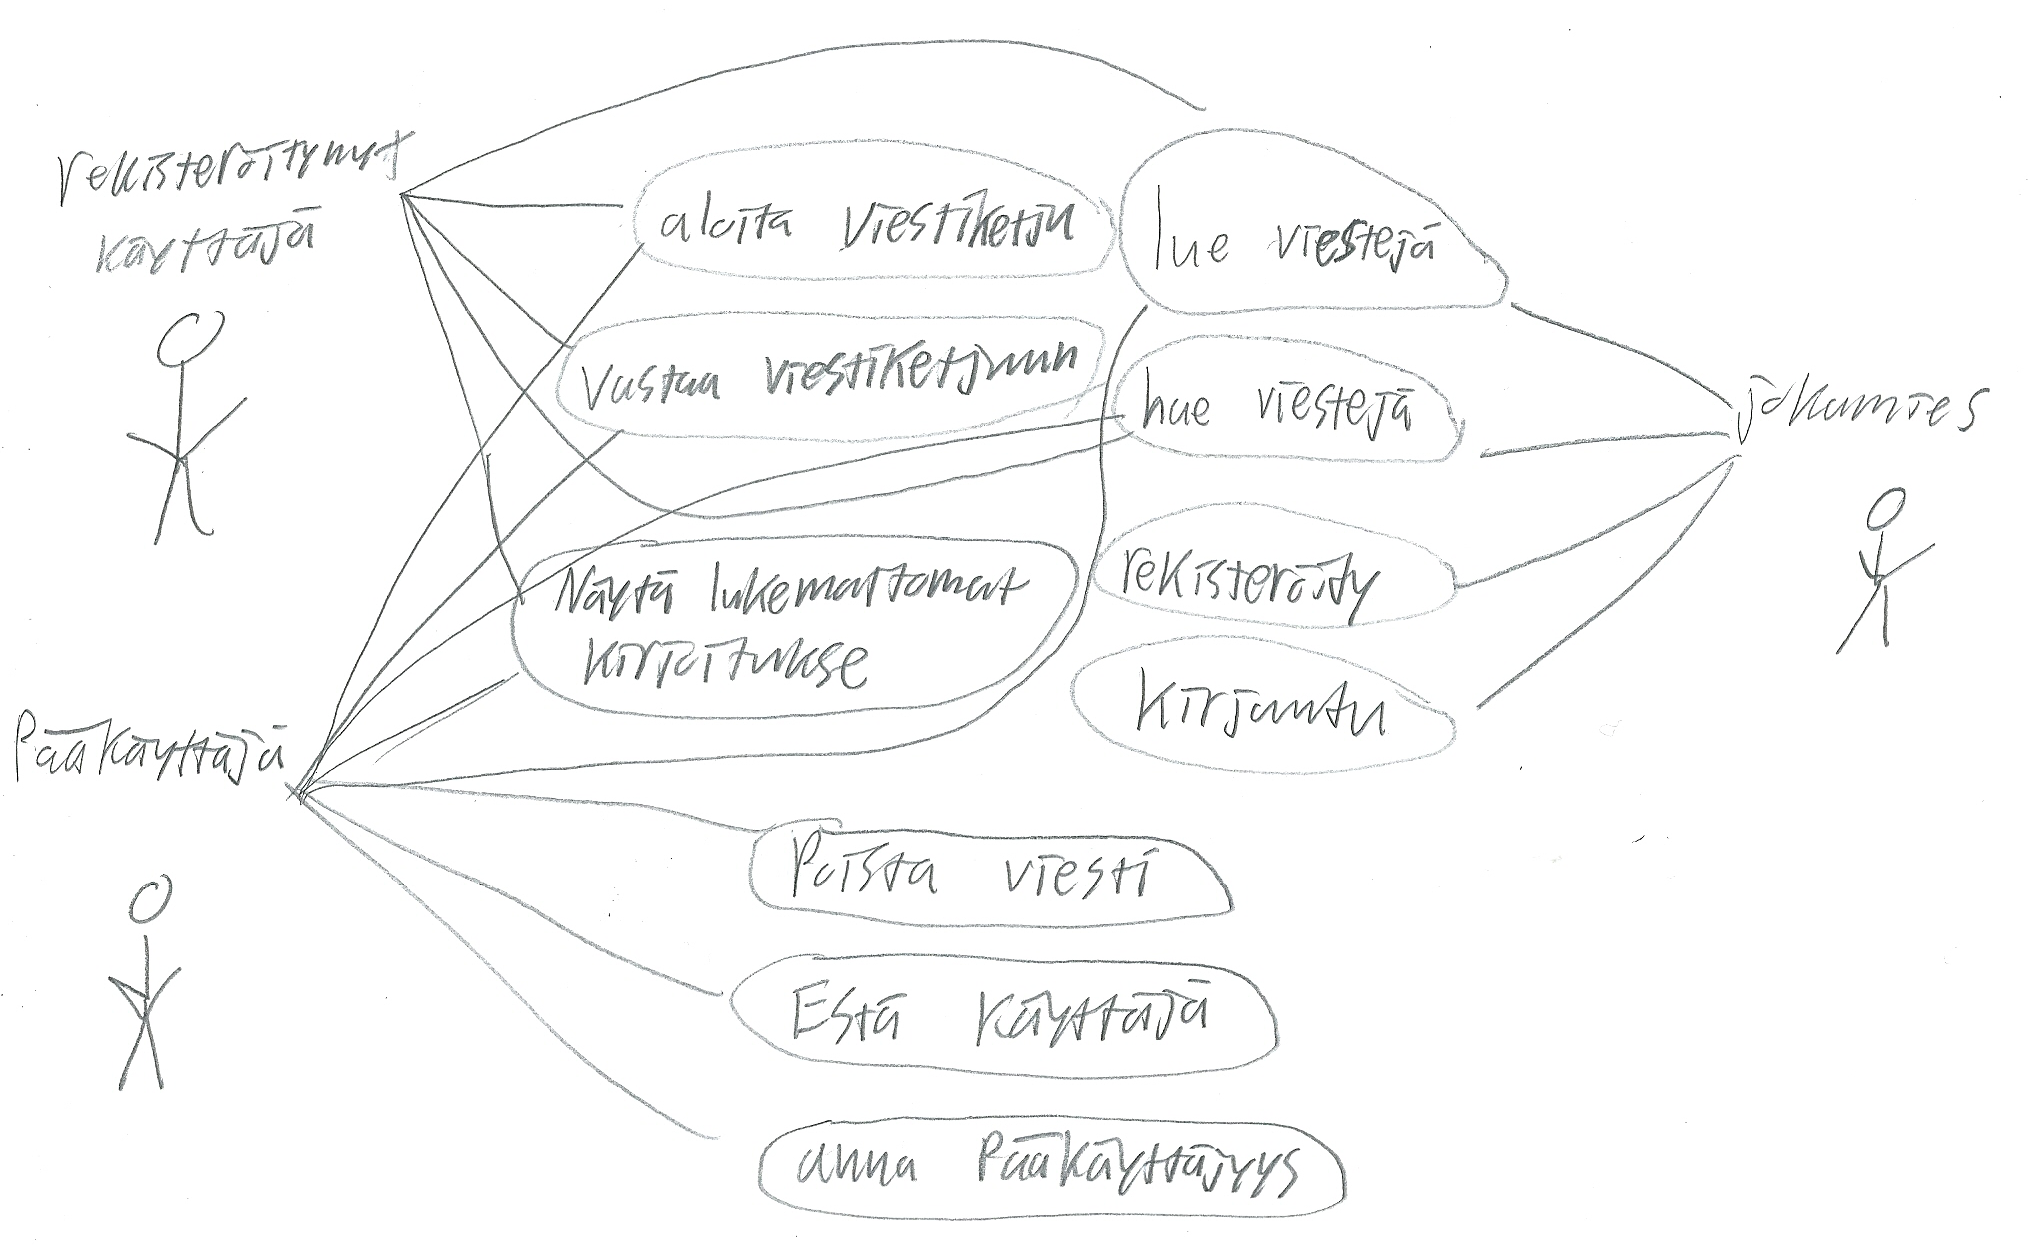
\includegraphics[width=\textwidth,height=\textheight,keepaspectratio]{kayttotapauskaavio.png}

\newpage

\section{Järjestelmän tietosisältö}
\subsection{Käsitekaavio}
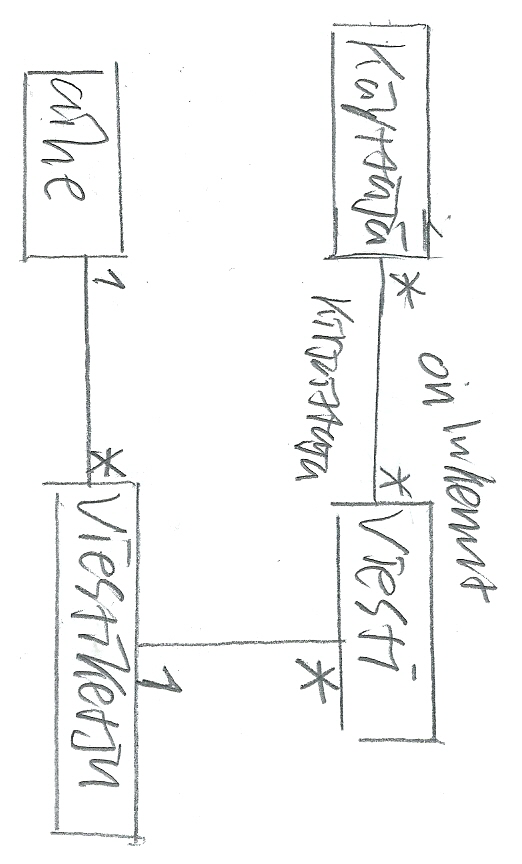
\includegraphics[width=\textwidth,height=\textheight,keepaspectratio]{kasitekaavio.png}

\subsection{Tietosisältö}
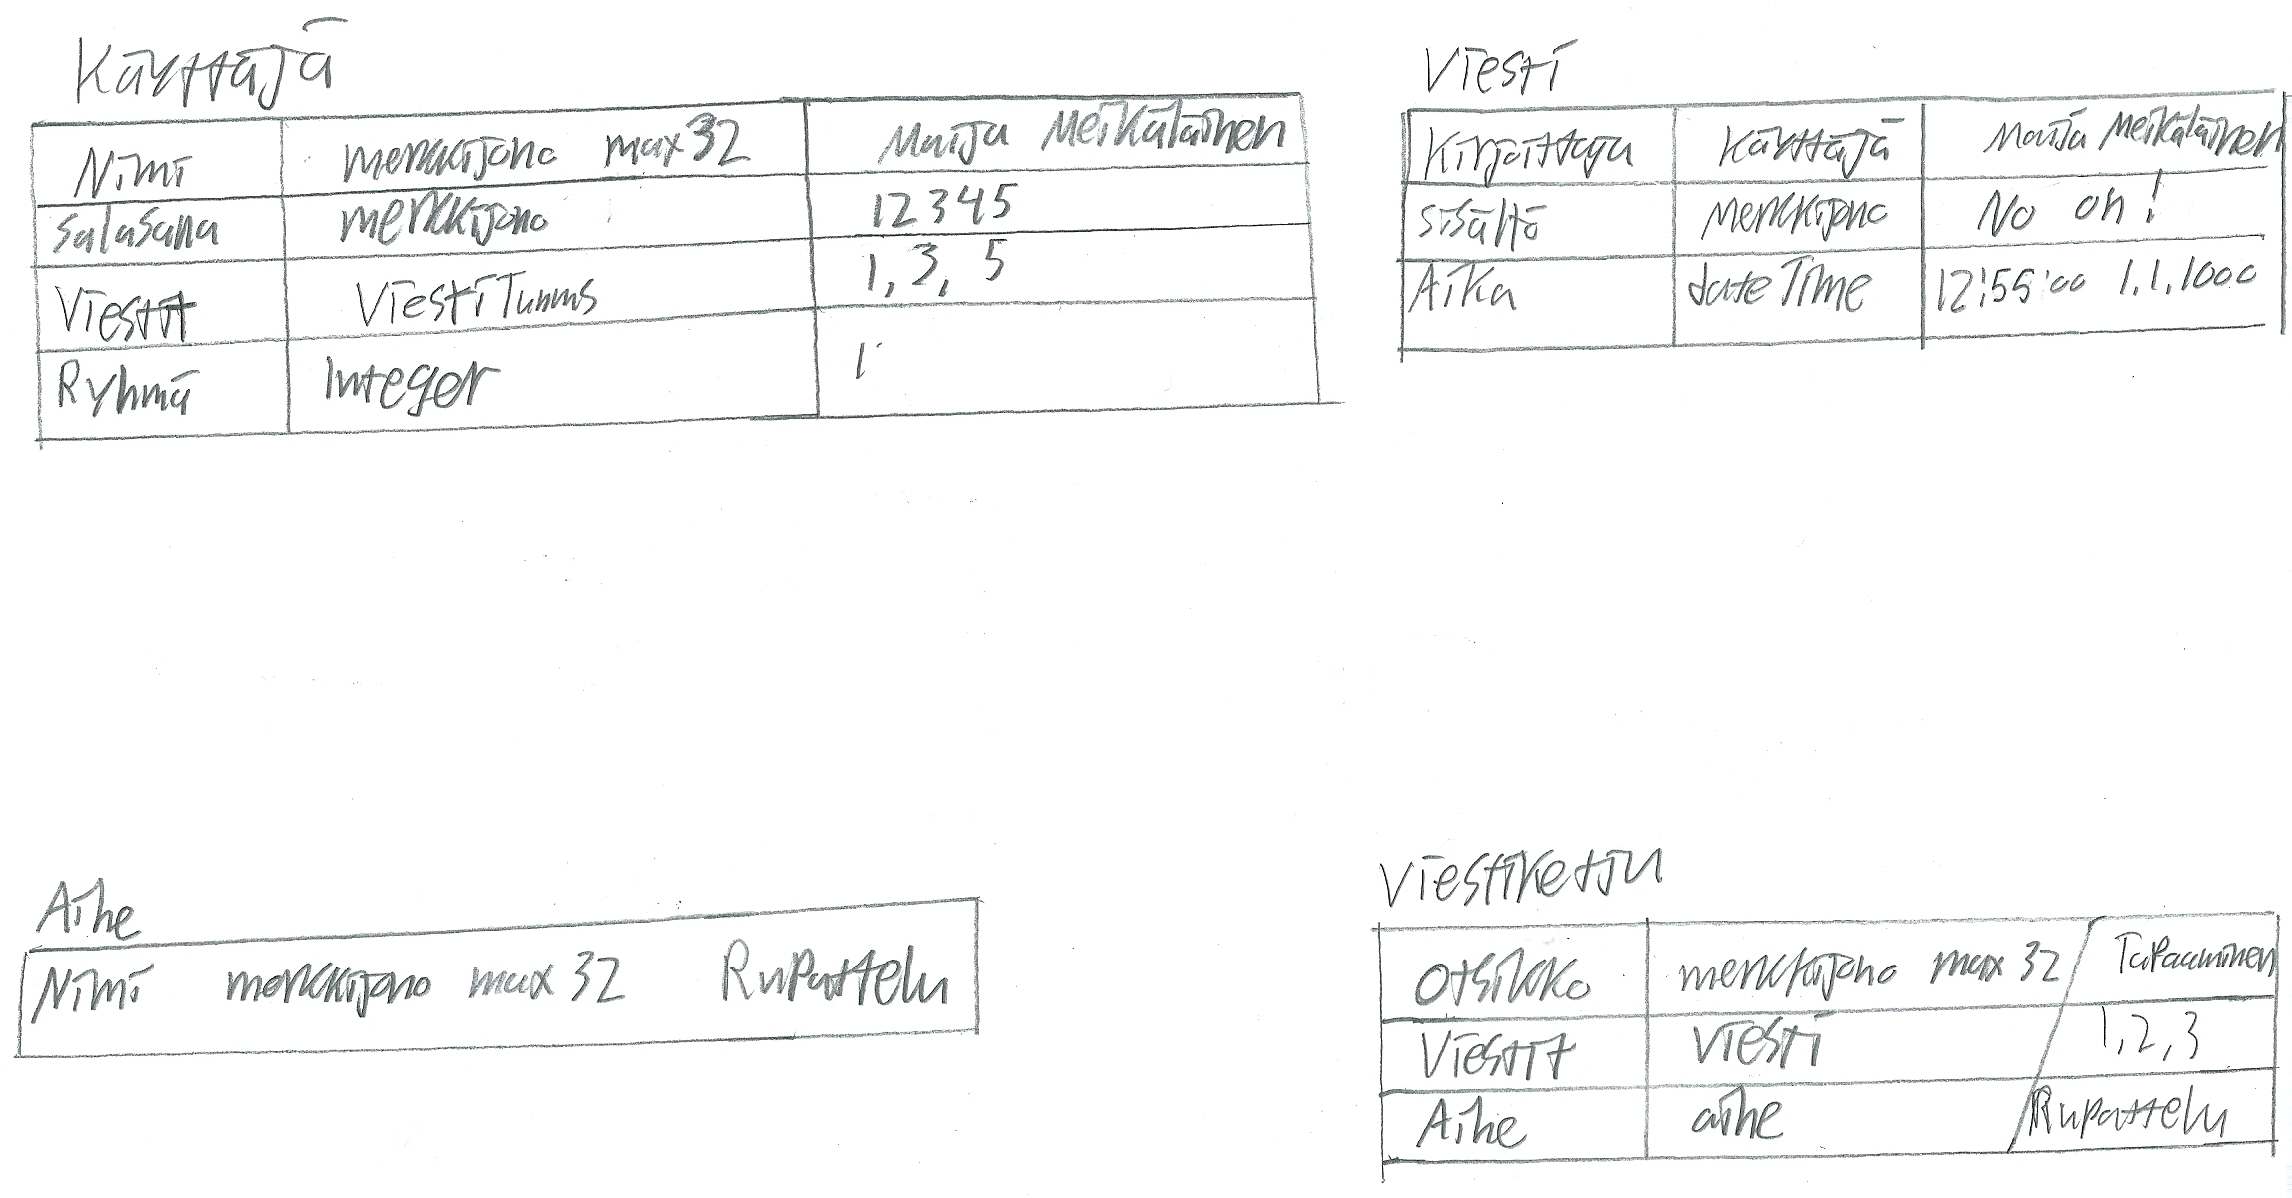
\includegraphics[width=\textwidth,height=\textheight,keepaspectratio]{tietosisalto.png}

\newpage

\section{Relaatiotietokantakaavio}
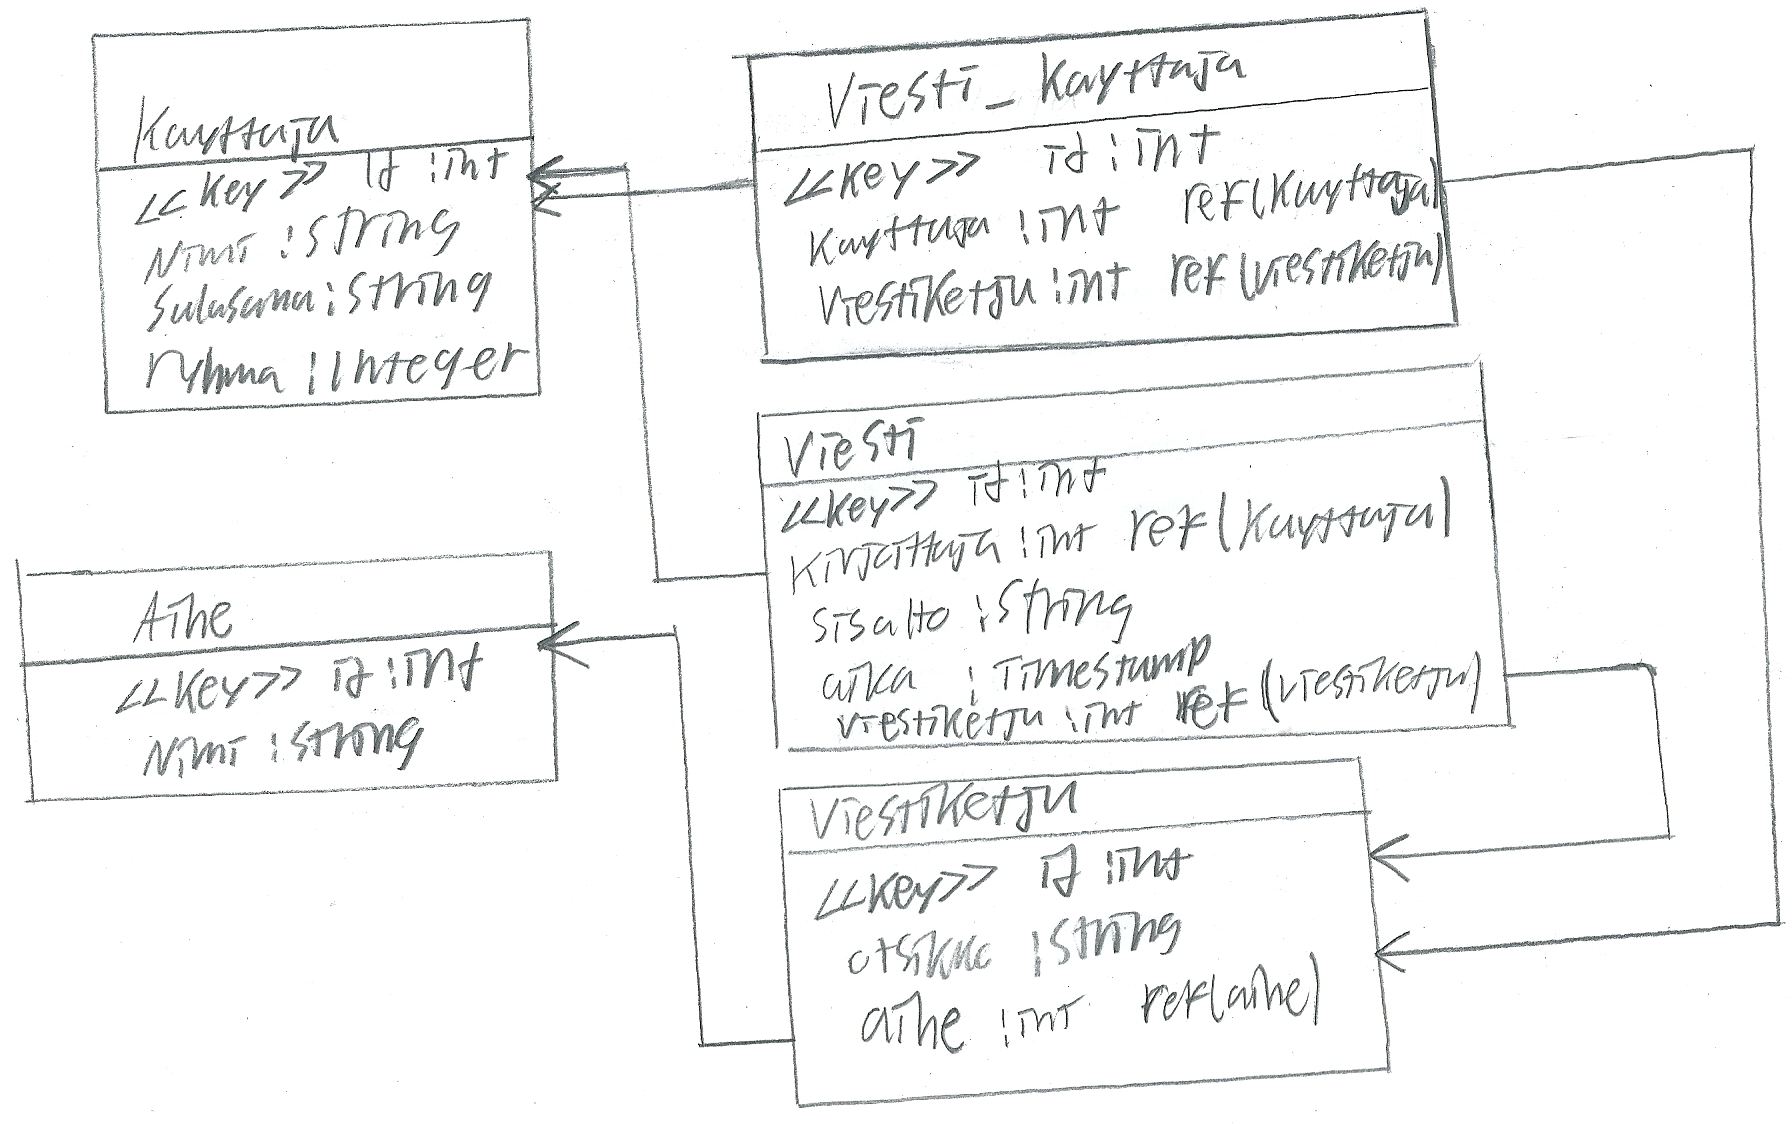
\includegraphics[width=\textwidth,height=\textheight,keepaspectratio]{relaatiotietokantakaavio.png}

\newpage

\section{Käyttöliittymä}
\subsection{Sivukartta}
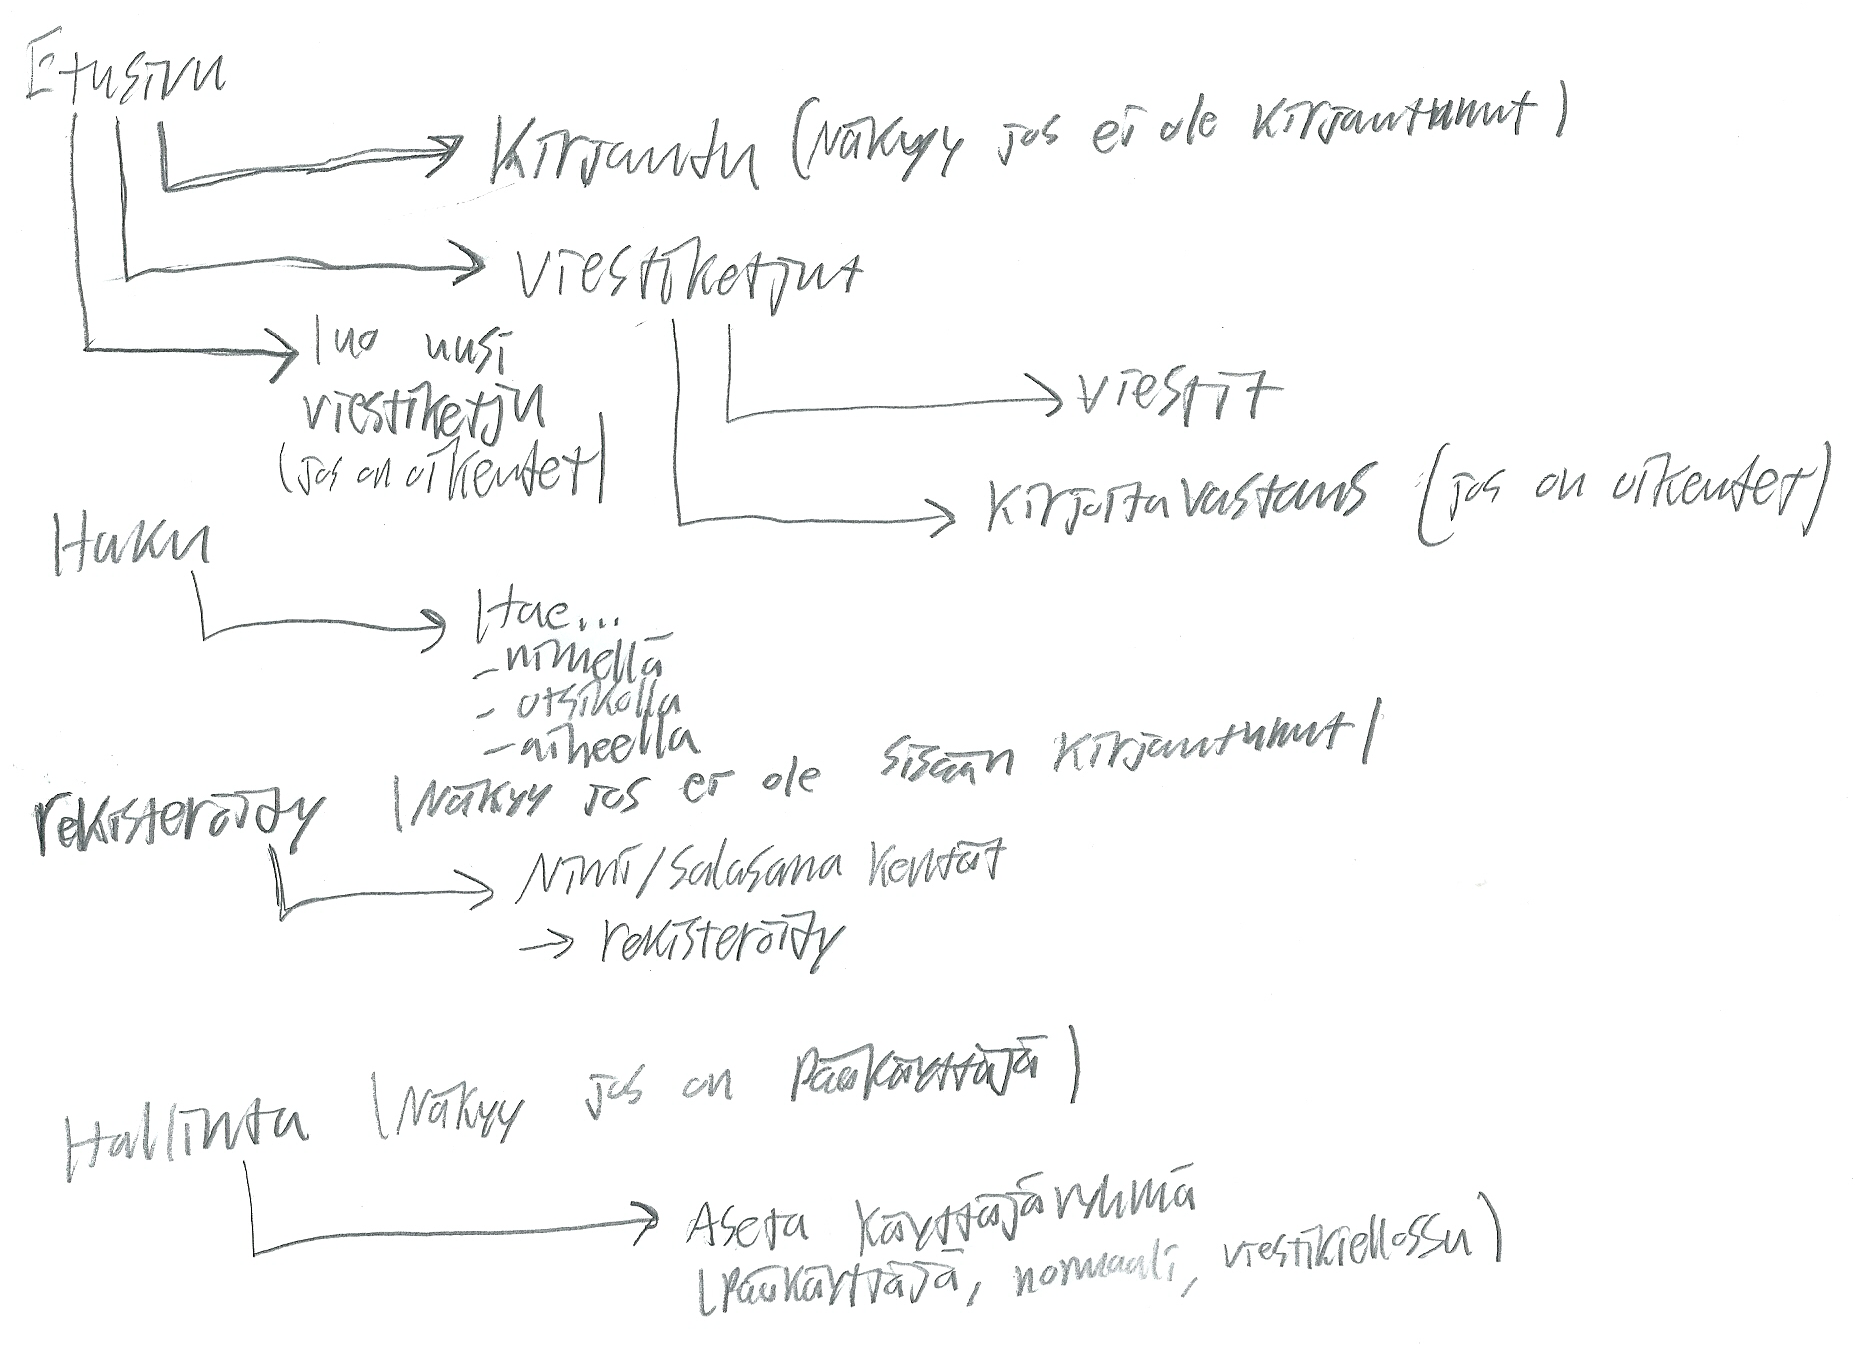
\includegraphics[width=\textwidth,height=\textheight,keepaspectratio]{kayttoliittymakaavio.png}

\subsection{Etusivu}
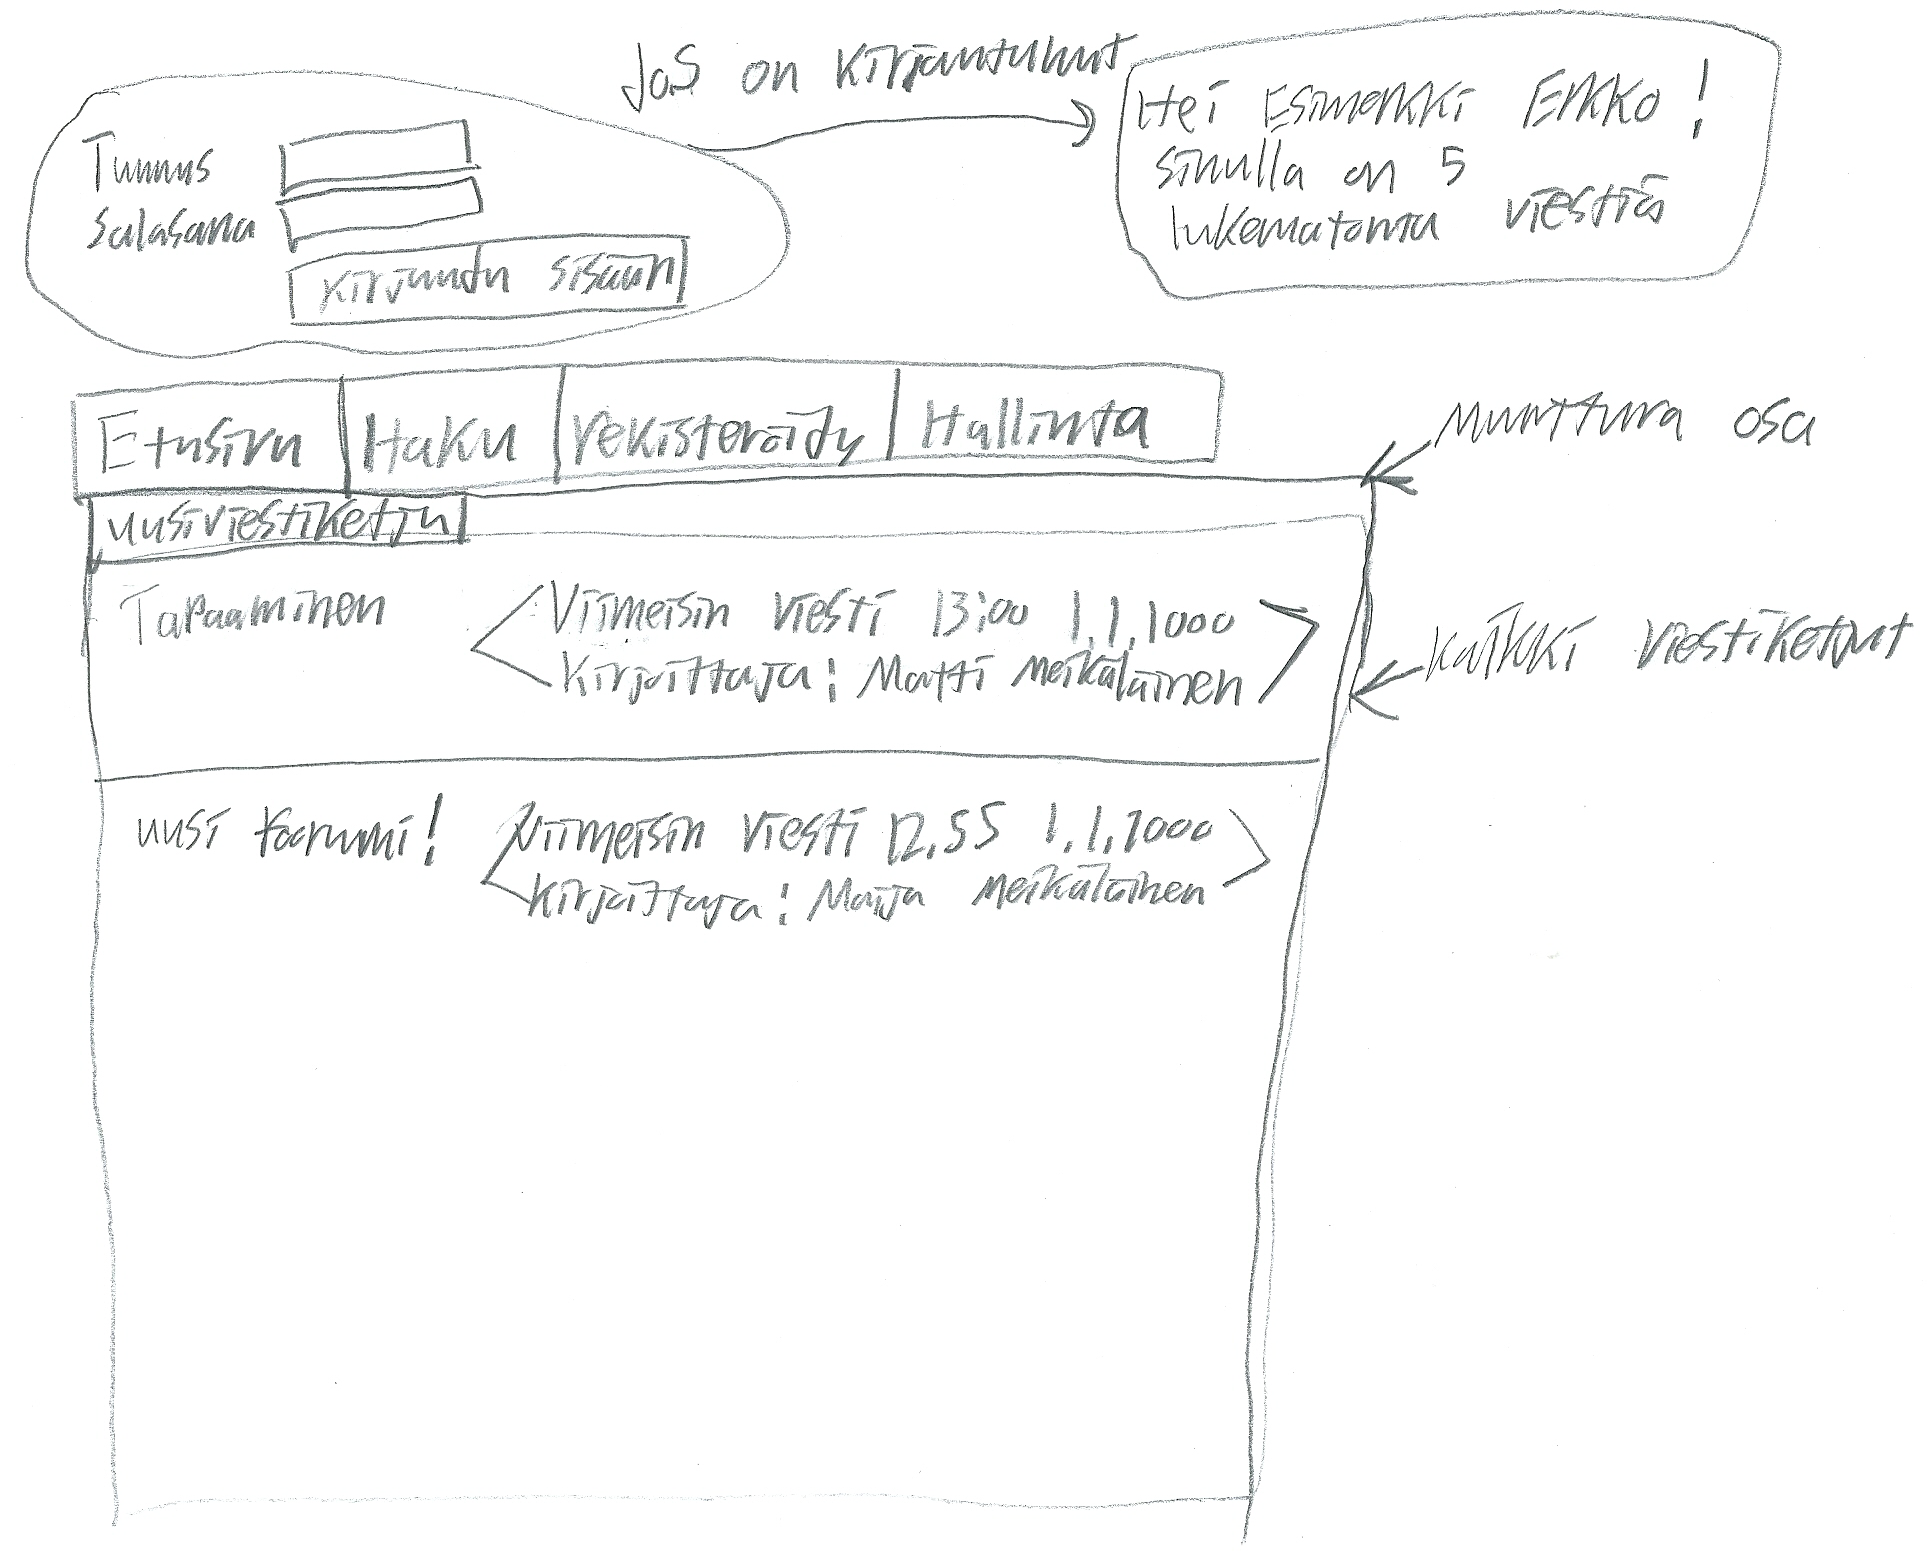
\includegraphics[width=\textwidth,height=\textheight,keepaspectratio]{etusivu.png}

\subsection{Haku}
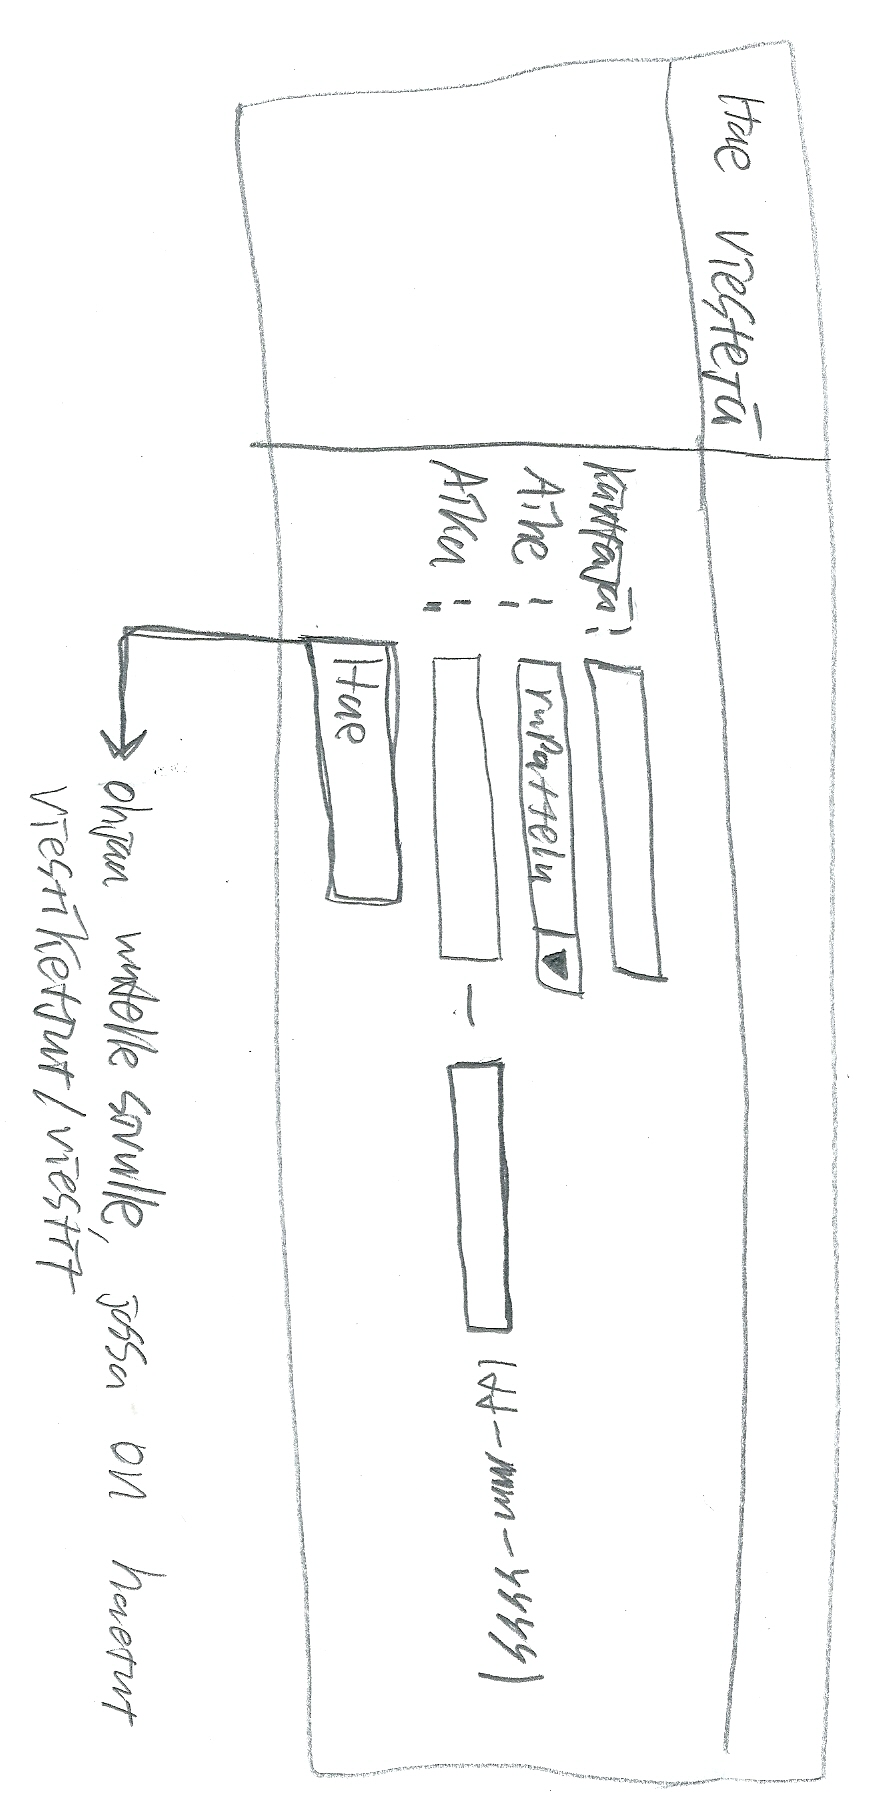
\includegraphics[width=\textwidth,height=\textheight,keepaspectratio]{haku.png}

\subsection{Hallinta}
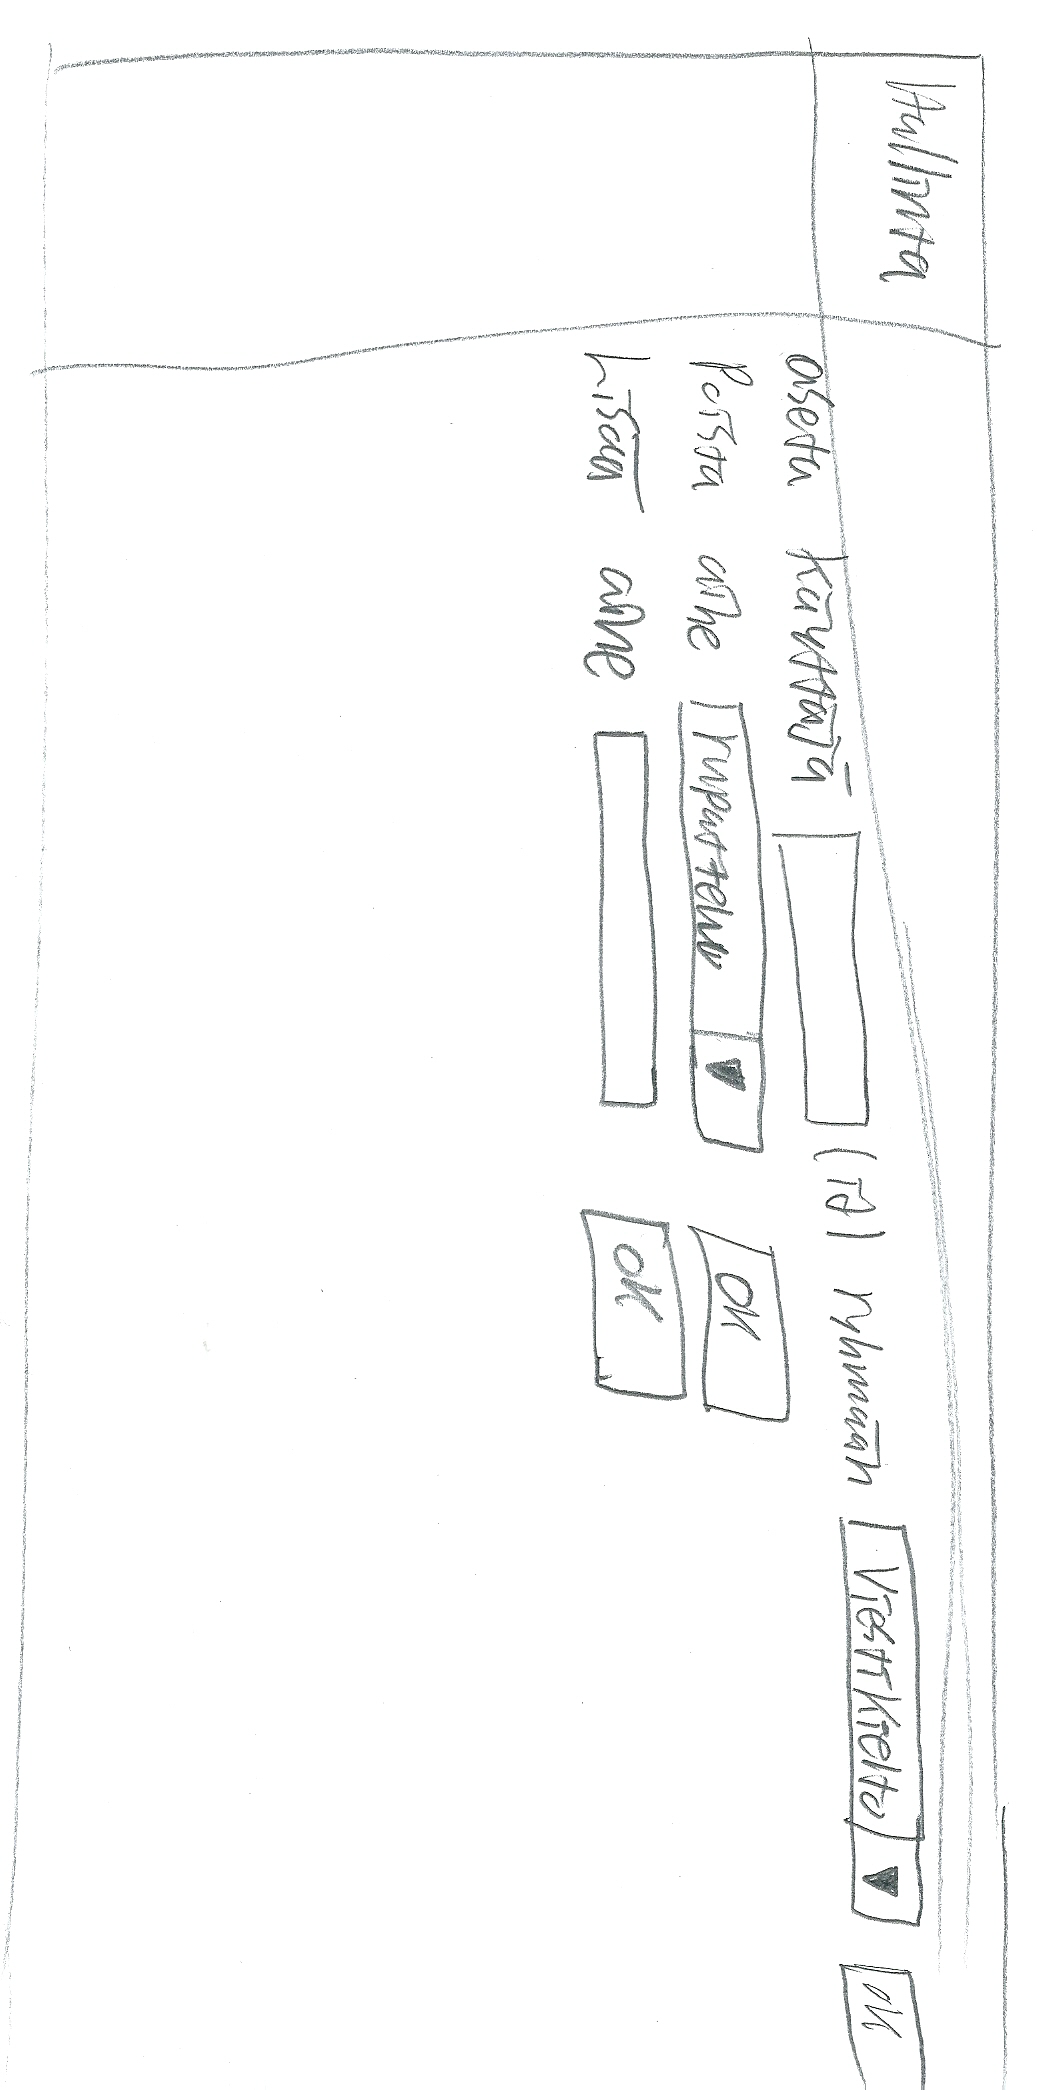
\includegraphics[width=\textwidth,height=\textheight,keepaspectratio]{hallinta.png}

\subsection{Rekisteröityminen}
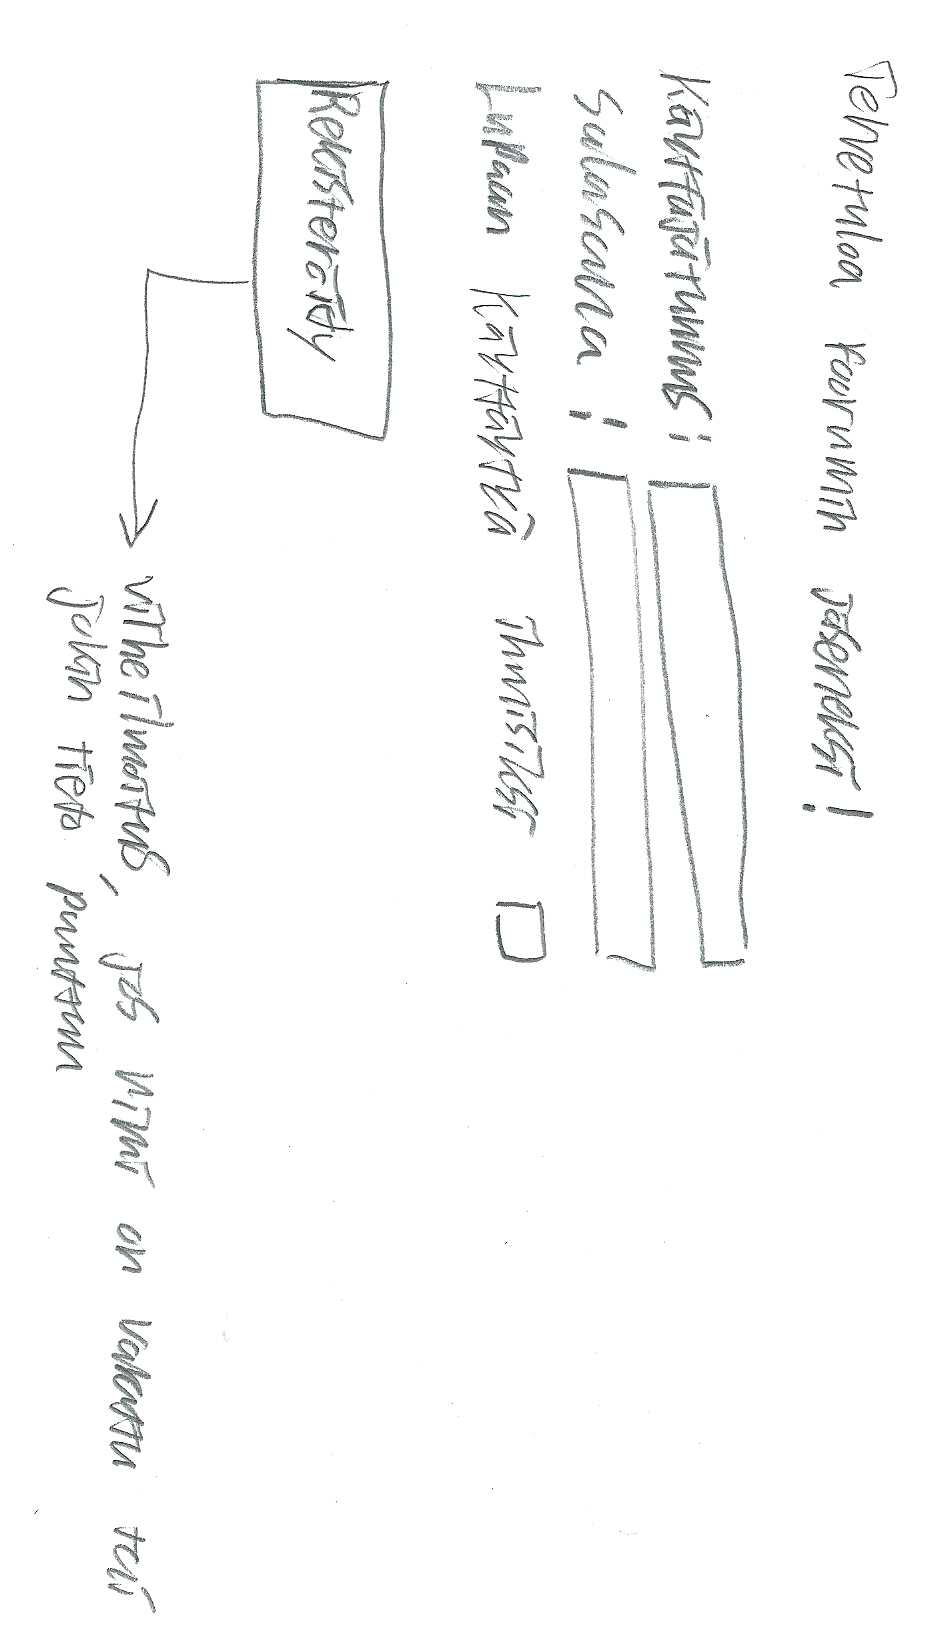
\includegraphics[width=\textwidth,height=\textheight,keepaspectratio]{rekisteroityminen.png}

\subsection{Uusiketju}
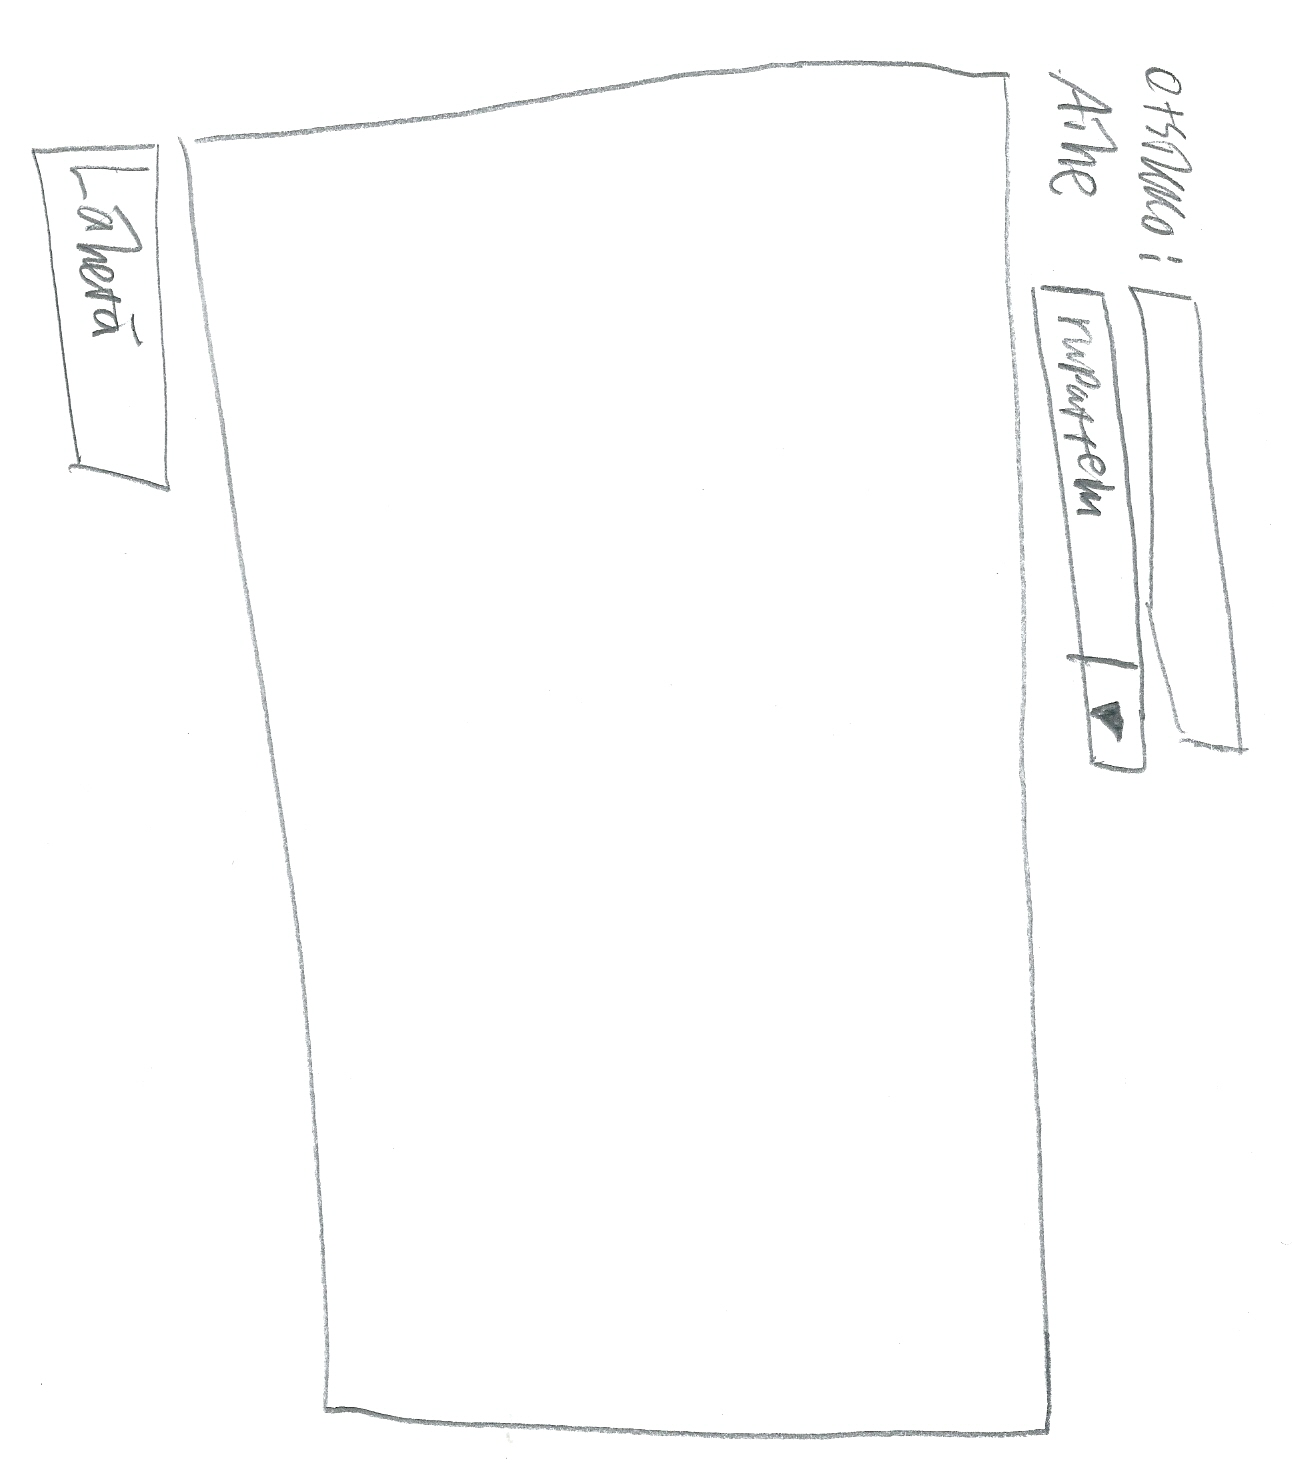
\includegraphics[width=\textwidth,height=\textheight,keepaspectratio]{uusiketju.png}

\subsection{Viestiketju}
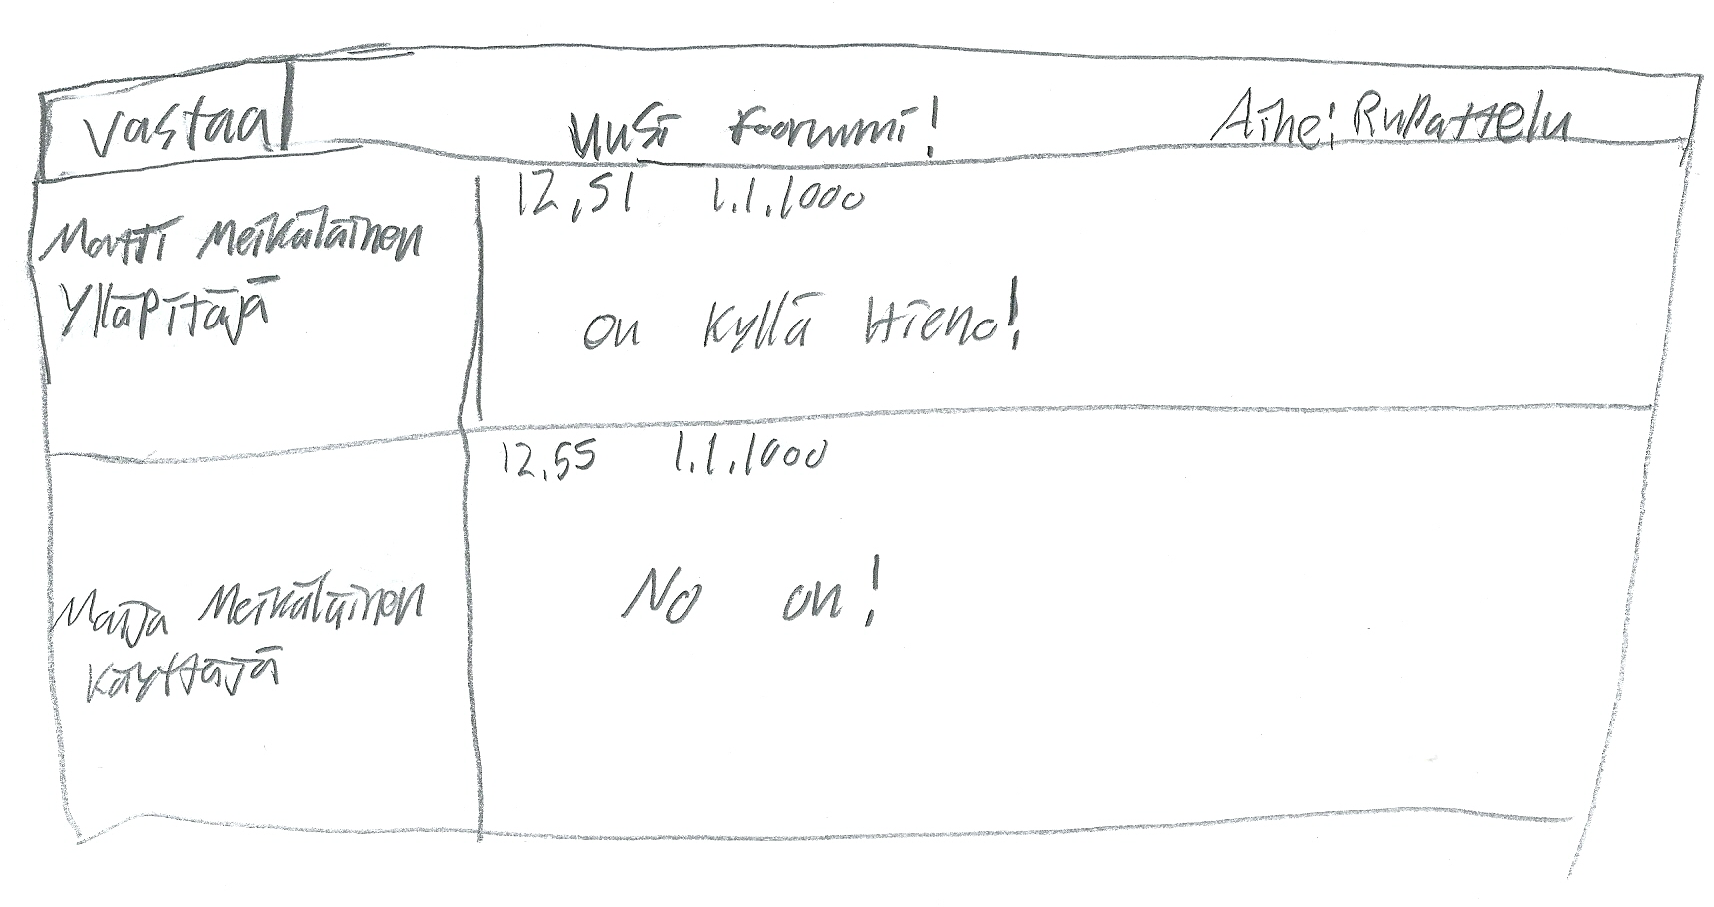
\includegraphics[width=\textwidth,height=\textheight,keepaspectratio]{viestiketju.png}

\subsection{Vastaus}
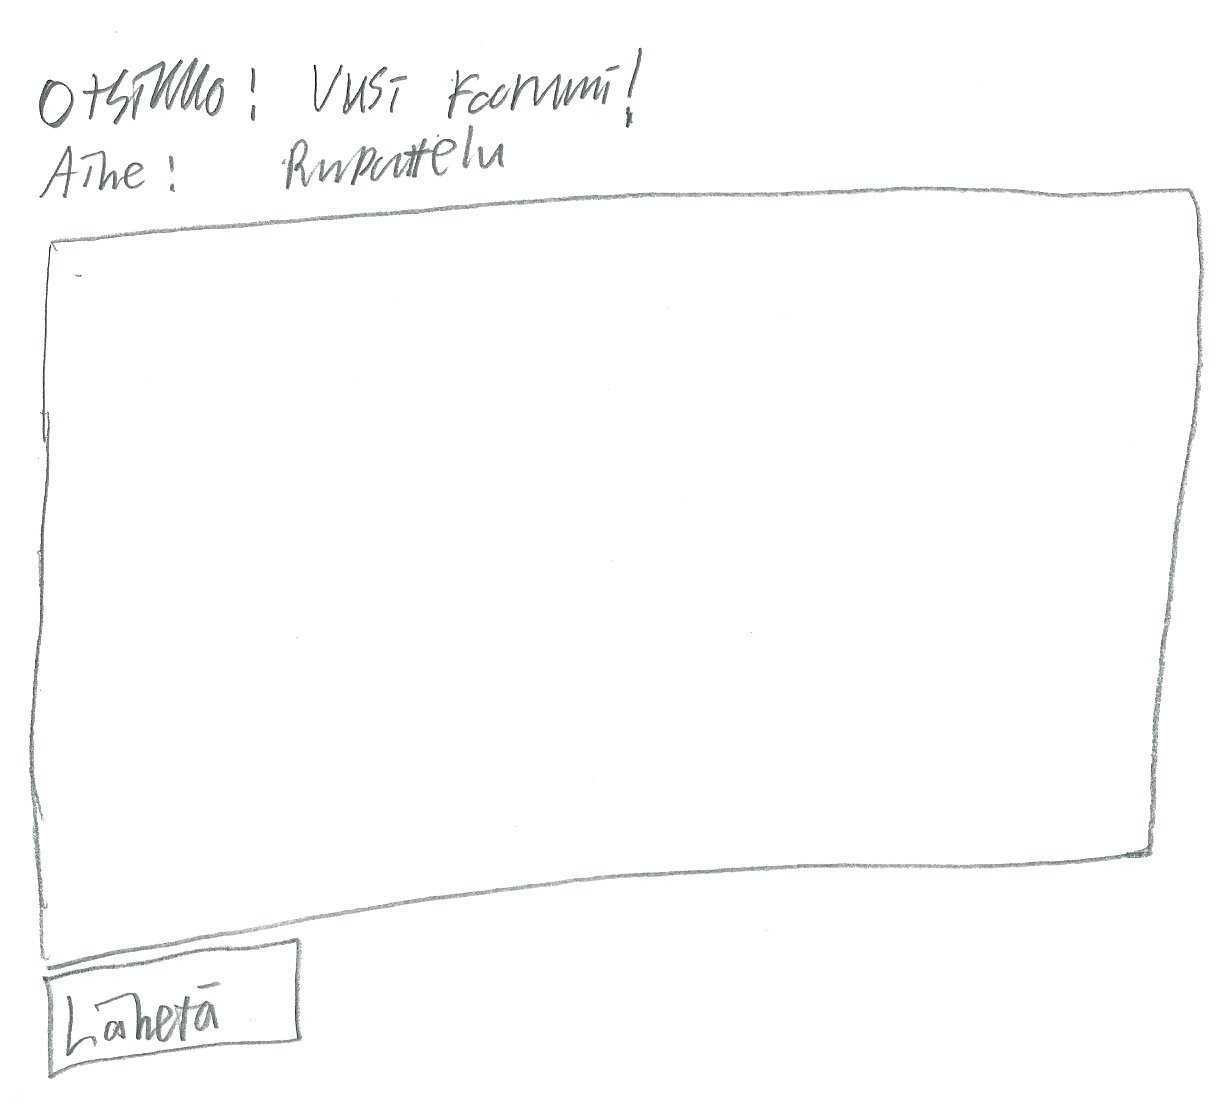
\includegraphics[width=\textwidth,height=\textheight,keepaspectratio]{vastaus.png}

\newpage

\section{Asennustiedot}
Foorumi on testattu PostgreSQL tietokannalla 8.4 sekä php 5.3:lla.
Foorumin asennus toteutetaan kopioimalla tiedostot johonkin näkyvään paikkaan, esimerkiksi kansioon htdocs.
Mitään salasanoja ei travitse laittaa, vaan users -palvelimella yhteys muodostetaan automaattisesti.
\indent

Kansiossa foorumi/sql on sql scriptit, joista osa pitää suorittaa ennen palvelimen käyttöönottoa.
create-tables.sql tulee suorittaa ensin.
add-test-data.sql vaaditaan, sillä foorumia ei ole testattu siten, että siinä ei ole mitään dataa.
Tämä scripti luo roskatietoa.
drop-tables.sql tuhoaa tietokannan sisällön. Tämän jälkeen create-tables.sql tulee suorittaa uudelleen.

\newpage

\section{Käyttöohjeet}
\begin{table}[ht]
\caption{Foorumin testitunnukset}
\centering
\begin{tabular}{c|c|c}
\hline
Nimi & Salasana & Rooli \\ [0.5ex]
\hline
NormiKäyttäjä&12345&Käyttäjä \\
Admin&admin&Ylläpitäjä \\
Käyttäjäkiellossa&666&Viestikiellossa \\ [1ex]
\hline
\end{tabular}
\end{table}

Kirjautuminen tapahtuu laittamalla tunnukset sivun yläosassa olevaan kirjautumislaatikkoon.
Kirjauduttua sisälle, käyttäjätunnuksen ja roolin tulisi näkyä kirjautumislaatikon tilalla.
\indent

Tällä hetkellä vain viestiketjuilla on täysi CRUD setti.
Niitä voi katsoa kuka tahansa ja niitä voivat rekisteröityneet käyttäjät luoda.
Ylläpitäjä voi muokata viestiketjujen aihetta tai otsikkoa.
Ylläpitäjä voi myös poistaa kokonaisia ketjuja.
Vaihtoehdot siihen tulevat viestikejun oikealle puolelle etusivulla.
Viestiketjuihin voi myös vastata.
\indent

Ylläpitäjä voi määritellä uusia aiheita ja poistaa vanhoja, olettaen että niihin ei liity viestiketjuja.
\indent

Ylläpitäjä voi myös asettaa käyttäjiä eriryhmiin.
Rekisteröitymällä pääsee käyttäjäryhmään.
\indent

Viestien muokkaus tapahtuu painamalla viestin oikealla alhaalla olevaa muokkaa painiketta.
\indent

Viestien haku vaatii kaikkien arvojen asettamista, eli sekä päiväys että käyttäjän nimi tulee olla.
Käyttäjän nimestä voi kirjoittaa vain osan ja senkin riippumatta isoista tai pienistä kirjaimista.
Päiväyksen ensimmäiseen kenttään tulee aikaisempi päiväys, toiseen myöhempi.
Viestit palautetaan niiden väliltä.

\newpage

\section{Järjestelmän yleisrakenne}
Järjestelmä on toteutettu MVC-mallin mukaisesti.
Controlleri on kaikkien sivujen yhteinen, mutta jokaisella sivulla on omia toimintoja jotka kuuluvat niiden omille sivuille.
Yleisesti yksittäisiltä sivuilta siirretään tieto array:ssa controllerille.
Controller luo pohjasivusta ilmentymän, johon liitetään kysytty sivu.
\indent

Kaikki tietokantayhteydet ovat vain tietokantayhteys.php:ssa.
Tietokantamallit ovat models kansiossa.
Malli luokat ovat toteutettu siten, että niitä luodaan staattisilla metodeilla.
Samoin toimii niiden tallennus.
\indent

Istuntoon tallennetaan käyttäjän kirjautuminen, virhe- ja onnistumisviestit.
Virhe- ja onnistumisviestit poistetaan istunnosta näytön jälkeen.
Kirjautuminen säilyy niin kauan kunnes käyttäjä kirjautuu ulos tai selain poistaa sen.
\indent

Käyttäjäoikeudet ovat models/groups kansiossa.
Käyttäjäryhmät toteuttavat kaikki ryhma -interfacen.
Jokainen käyttäjäryhmä luokka toteuttaa käyttöoikeuksia virtuaalisilla metodeilla, sekä sivujen katsomisoikeudet arraylla.
Sivujen katsomisoikeudet toimivat siten, että ellei erikseen ole ryhmälle lupaa nähdä sivua, sitä ei näytetä.

\newpage

\section{Käyttöliittymä ja järjestelmän komponentit}
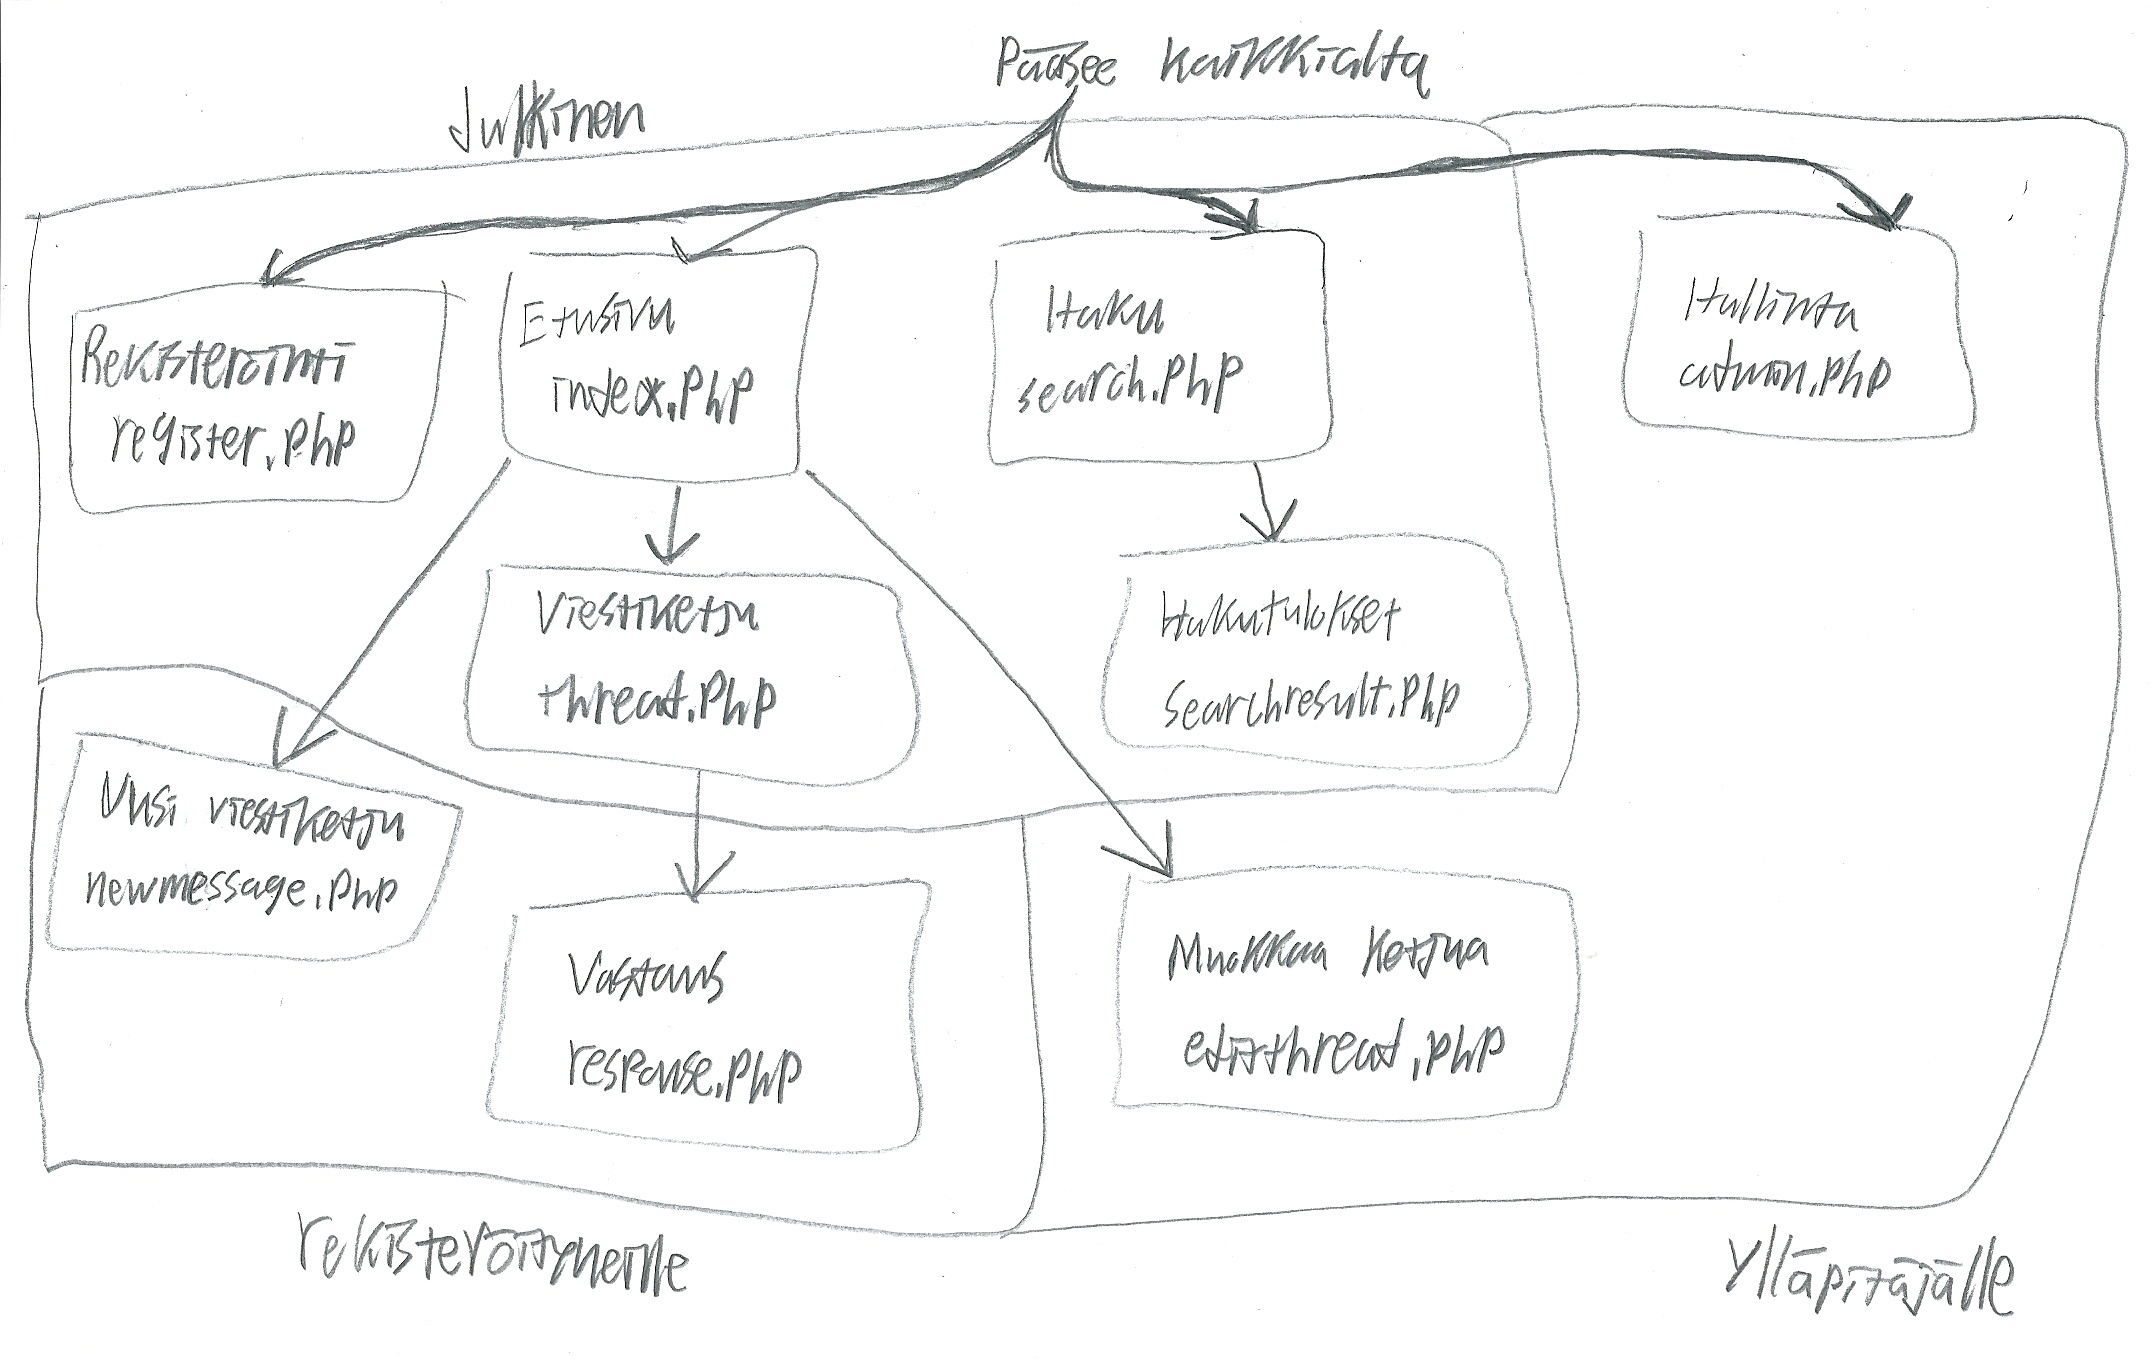
\includegraphics[width=\textwidth,height=\textheight,keepaspectratio]{kayttoliittyma.png}

\newpage

\section{Testaus, tunnetut bugit ja puutteet, jatkokehitysideat}
Tunnettuja bugeja ei ole.
Foorumi on hyvin yksinkertainen, joten puutteet ovat ominaisuuksia.
Ohjelmistossa ei ole automaattista testausta, vaan kaikkea on testattu käsin.
Jatkokehitysideoita:
\begin{itemize}
\item
Viestien poisto
\item
Viestien haku ilman että kaikkia kenttiä tarvitsee täyttää
\item
Alemman pääkäyttäjän rooli, voisi esimerkiksi vain poistaa ja muokkaa viestejä
\item
Viestiketjujen lukitseminen
\item
Käyttäjän omat sivut, esimerkiksi yhteystiedot ja aikavyöhyke
\item
Yksityiset viestit
\item
Viestit omiin "kansioihin" aiheiden perusteella, helpottamaan selausta
\end{itemize}

\end{document}
